\section{Introduction}

%\paragraph{Motivation}

Simultaneously imaging large populations of neurons using calcium sensors is becoming increasingly popular \cite{ImagingManual}, both in vitro \cite{SmettersYuste99, IkegayaYuste04} and in vivo \cite{NagayamaChen07, GobelHelmchen07, LuoSvoboda08}, and is expected to continue as the signal-to-noise-ratio (SNR) of genetic sensors continues to improve \cite{GaraschukKonnerth07, MankGriesbeck08, WallaceHasan08}. 
Whereas the data from these experiments are movies of time-varying fluorescence traces, the desired signal is typically the spike trains of the observable neurons. Unfortunately, finding the most likely spike train is a challenging computational task, due to poor SNR, poor temporal resolution, unknown parameters, and computational intractability. One is therefore effectively forced to find an approximately most likely spike train, or hope that the inferred spike train is indeed most likely. 

A number of groups have therefore proposed algorithms to infer spike trains from calcium fluorescence data.  For instance, Greenberg et al. \cite{GreenbergKerr08} developed a novel template matching algorithm. %, which performed well on their data, but is not particularly computationally efficient
Holekamp et al. \cite{HolekampHoly08} took a very different strategy, by performing the optimal linear deconvolution (ie, the Wiener filter) on the fluorescence data.  This approach is natural from a signal processing standpoint, but does not utilize the knowledge that spikes are always positive.  Vogelstein et al. \cite{VogelsteinPaninski09} proposed a sequential Monte Carlo method to efficiently estimate the probability of a spike in each image frame, given the entire fluorescence time-series.  While effective, that approach is not suitable for online analyses of populations of neurons, as the computations run in about real-time per neuron (ie, analyzing one minute of data requires about one minute of computational time on a standard laptop computer).

The present work starts by building a generative model relating spiking activity to fluorescence traces. Unfortunately, inferring the most likely spike train given this model is computationally intractable.  Making some reasonable approximations leads to an algorithm that infers the approximately most likely spike train, given the fluorescence data.  This algorithm has a few particularly noteworthy features, relative to other approaches.  First, spikes are assumed to be positive.  This assumption often improves filtering results when the underlying signal has this property \cite{PortugalVicente94, MarkhamConchello99, LeeSeung99, LLS04, OGradyPearlmutter06, HuysPaninski06, Cunningham08, PaninskiWu09}.  Second, the algorithm is extremely fast: it can process a calcium trace from 50,000 images in about one second on a standard laptop computer. In fact, filtering the signals for an entire population of about $100$ neurons runs in super-real-time (ie, \emph{faster} than real-time). This speed facilitates using this filter online, as observations are being collected. In addition to these two features, the model may be generalized in a number of ways, including incorporating spatial filtering of the raw movie. The efficacy of the proposed filter is demonstrated on several real data-sets, suggesting this algorithm is a powerful and robust tool for online spike train inference.  The code (which is a simple Matlab script) is available from the authors upon request.







\section{Methods} \label{sec:methods}

%As mentioned above, starting with an in vitro experiment, for which the SNR is relatively high, an appropriate generative model can be built (section \ref{sec:model}).  Given this model, a goal can be formalized (section \ref{sec:goal}).  And given this goal, an approximately optimal inference algorithm is derived (section \ref{sec:inf}) .  This algorithm depends on a number of unknown parameters, which can be estimated directly from the fluorescence observations (section \ref{sec:learn}).  The effective signal-to-noise ratio (SNR) of the fluorescence trace can be potentially improved by spatially filtering the movie (section \ref{sec:methods:spatial}), even when multiple neurons are within a region-of-interest (ROI) (section \ref{sec:methods:overlapping}).  


\subsection{Data driven generative model} \label{sec:model}

Figure \ref{fig:in_vitro_ex} shows data from a typical in vitro, epifluorescence experiment (see section \ref{sec:exp} for data collection details).  The top panel shows the mean frame of this movie, including 3 neurons, two of which are patched.  To build the model, the pixels within a region-of-interest (ROI) are selected (white circle).  Given the ROI, all the pixel intensities of each frame can be averaged, to get a one-dimensional fluorescence time-series, as shown in the bottom left panel (black line).  By patching onto this neuron, the spike train can also be directly observed (black bars). Previous work suggests that this fluorescence signal might be well characterized by convolving the spike train with an exponential, and adding noise \cite{ImagingManual}.  This model is confirmed by convolving the true spike train with an exponential (gray line, bottom left panel), and then looking at the distribution of the residuals.  The bottom right panel shows a histogram of the residuals (black line), and the best fit Gaussian distribution (gray line).


\begin{figure}[h!]
\centering 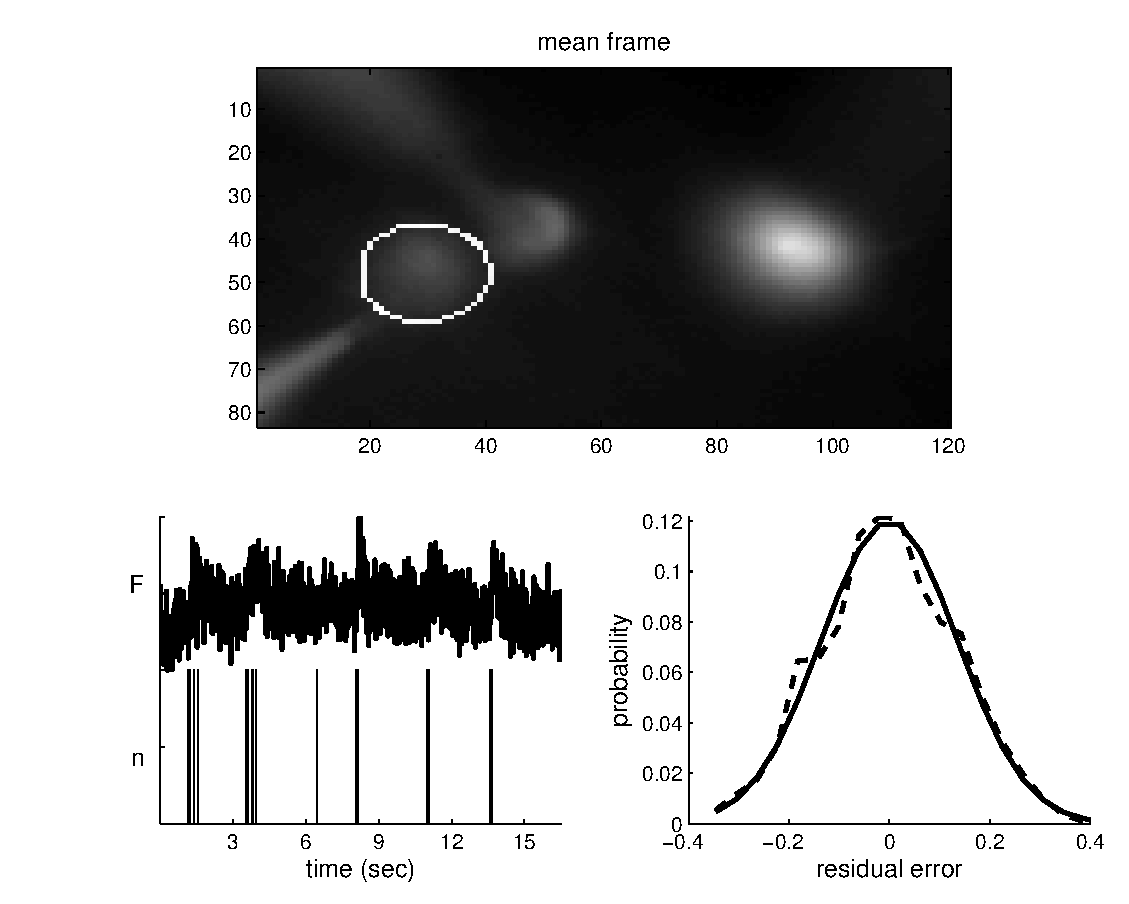
\includegraphics[width=.9\linewidth]{/Users/joshyv/Research/oopsi/fast-oopsi/figs/in_vitro_ex}
\caption[data-based model]{Typical in vitro data suggest that a reasonable first order model may be constructed by convolving the spike train with an exponential, and adding Gaussian noise. Top panel: the average (over frames) of a typical field-of-view.  Bottom left: spike train (black bars), convolved with an exponential (gray line), superimposed on the one-dimensional fluorescence time-series (black line).  Bottom right: a histogram of the residual error between the gray and black lines from the bottom left panel (black line), and the best fit Gaussian (gray line).} \label{fig:in_vitro_ex}
\end{figure}

The above observations may be formalized as follows. Assume there is a one-dimensional fluorescence trace, $\bF$ (throughout this text $\bX$ indicates the vector $(X_1, \ldots, X_T)$, where $T$ is the index of the final frame), from a neuron.  At time $t$, the fluorescence measurement, $F_t$ is a linear-Gaussian function of the intracellular calcium concentration at that time, $\Ca_t$:
\begin{align} \label{eq:F}
F_t &= \alpha (\Ca_t + \beta) + \sig \varepsilon_t, \qquad \varepsilon_t \overset{iid}{\sim} \mN(0,1).
\end{align}
\noindent The scale, $\alpha$, absorbs all experimental variables impacting the scale of the signal, including number of sensors within the cell, photons per calcium ion, amplification of imaging system, etc.  Similarly, the offset, $\beta$, absorbs baseline calcium concentration of the cell, background fluorescence of the fluorophore, imaging system offset, etc.  The standard deviation, $\sig$, results from calcium fluctuations independent of spiking activity, fluorescence fluctuations independent of calcium, and imaging noise. The noise at each time, $\varepsilon_t$, is independently and identically distributed according to a standard normal distribution (ie, Gaussian with zero mean and unit variance), as indicated by the notation $\overset{iid}{\sim}\mN(0,1)$. 

Then, assuming that the intracellular calcium concentration, $\Ca_t$, jumps by $A$ $\mu$M after each spike, and subsequently decays back down to $C_b$ $\mu$M with time constant, $\tau$, one can write:
\begin{align} \label{eq:C1}
[\Ca_{t+\Del} = (1- \Del/\tau ) \Ca_t + C_b + A n_t
\end{align}
\noindent where $\Del$ is the time step size --- which is the frame duration, or $1/$(frame rate) --- and $n_t$ indicates the number of times the neuron spiked in frame $t$. %, and $\gam=1-\Del/\tau$. \footnote{This follows from writing \eqref{eq:C} as $\tau \frac{C_t - C_{t-1}}{\Del} = -C_{t-1} + n_t$.} 
Note that because $\Ca_t$ and $F_t$ are linearly related to one another, the fluorescence scale, $\alpha$, and calcium scale, $A$, are not identifiable.  In other words, either can be set to unity without loss of generality, as the other can absorb the scale entirely. Similarly, the fluorescence offset, $\beta$, and calcium baseline, $C_b$ are not identifiable, so either can be set to zero without loss of generality.  Finally, letting $\gam=(1-\Del/\tau)$, Eq.~\eqref{eq:C1} can be rewritten replacing $\Ca_t$ with its non-dimensionalized counterpart, $C_t$: 
\begin{align} \label{eq:C2}
	 C_{t+\Del}=\gam C_t + n_t.
\end{align} 
\noindent Note that $C_t$ does not refer to absolute intracellular concentration of calcium, but rather, a relative measure (but see \cite{VogelsteinPaninski09} for a more general model).  The gray line in the bottom left panel of Figure \ref{fig:in_vitro_ex} corresponds to the putative $\bC$ of the observed neuron.  

To complete the ``generative model'' (ie, a model from which simulations can be generated), the distribution from which spikes are sampled must be defined.  Perhaps the simplest first order description of spike trains is that at each time, spikes are sampled according to a Poisson distribution with some rate:
\begin{align} \label{eq:n}
	n_t \overset{iid}{\sim} \text{Poisson}(\lam \Del)
\end{align}
\noindent where $\lam \Del$ is the expected firing rate, and $\Del$ is included to ensure that the expected firing rate is independent of the frame rate.  Thus, Eqs.~\eqref{eq:F}, \eqref{eq:C2}, and \eqref{eq:n} complete the generative model.  






\subsection{Goal} \label{sec:goal}

Given the above model, the goal is to find the maximum \emph{a posteriori} (MAP) spike train, ie, the most likely spike train, $\hbn$,  given the fluorescence measurements, $\bF$:
\begin{align} \label{eq:nhat1} 
\hbn &=  \anx P[\bn | \bF], 
\end{align}
\noindent where $P[\bn | \bF]$ is the posterior probability of a spike train, $\bn$, given the fluorescent trace, $\bF$, and $n_t$ is constrained to be an integer, $\mathbb{N}_0=\{0,1,2,\ldots\}$, because of the above assumed Poisson distribution.  From Bayes' Rule, the posterior can be rewritten:
\begin{align} \label{eq:bayes}
P[\bn | \bF] = \frac{P[\bn, \bF]}{P[\bF]} = \frac{1}{P[\bF]} P[\bF | \bn] P[\bn],
\end{align}
\noindent where $P[\bF]$ is the evidence of the data, $P[\bF | \bn]$ is the likelihood of observing a particular fluorescence trace $\bF$, given the spike train $\bn$, and $P[\bn]$ is the prior probability of a spike train.  Plugging the far right-hand-side of Eq.~\eqref{eq:bayes} into Eq.~\eqref{eq:nhat1}, yields:
\begin{align} \label{eq:nhat2} 
\hbn &=  \anx \frac{1}{P[\bF]} P[\bF | \bn] P[\bn] =  \anx  P[\bF | \bn] P[\bn],
\end{align}
\noindent where the second equality follows because $P[\bF]$ merely scales the results, but does not change the relative quality of various spike trains.  Fortunately, both $P[\bF | \bn]$ and $P[\bn]$ are available from the above model:
\begin{subequations} \label{eq:post1}
\begin{align}
P[\bF | \bn]&= P[\bF | \bC] 	= \prod_{t=1}^T P[F_t | C_t], \label{eq:lik1} \\ 
P[\bn] 		&= \prod_{t=1}^T P[n_t], \label{eq:prior1}
\end{align}
\end{subequations}
\noindent where the first equality in Eq.~\eqref{eq:lik1} follows because $\bC$ is deterministic given $\bn$, and the second equality follows from Eq.~\eqref{eq:F}. Further, Eq.~\eqref{eq:prior1} follows from the Poisson process assumption, Eq.~\eqref{eq:n}.  Both $P[F_t | C_t]$ and $P[n_t]$ can be written explicitly:
\begin{subequations} \label{eq:post2}
\begin{align}
P[F_t | C_t] &= \mN(\alpha(C_t+\beta),\sig^2), \label{eq:lik2} \\
P[n_t] &= \text{Poisson}(\lam \Del), \label{eq:prior2} 
\end{align}
\end{subequations}
%\noindent where $\mN(x;\mu,\sig^2)$ indicates $x$ has a Gaussian distribution with mean $\mu$ and variance $\sig^2$ and Poisson$(x;r)$ indicates that $x$ has a Poisson distribution with rate $r$, and 
where both equations follow from the above model.  Now, plugging Eq.~\eqref{eq:post2} back into \eqref{eq:post1}, and plugging that result into Eq.~\eqref{eq:nhat2}, yields:
\begin{subequations}  \label{eq:obj}
\begin{align}
\hbn 	&= \anx \prod_{t=1}^T \frac{1}{\sqrt{2 \pi \sig^2}} \exp \left\{-\frac{1}{2}\frac{(F_t - \alpha (C_t + \beta))^2}{\sig^2}\right\} \frac{\exp\{-\lam\Del\} (\lam\Del)^{n_t}}{n_t!}
\label{eq:obj1}\\ &= \anx  \sum_{t=1}^T \bigg( -\frac{1}{2 \sig^2}(F_t - \alpha(C_t + \beta))^2  +  n_t \log \lam \Del - \log n_t! \bigg), \label{eq:logobj1}
\end{align} 
\end{subequations}
\noindent where the second equality follows from taking the logarithm of the right-hand-side.  Unfortunately, solving Eq.~\eqref{eq:logobj1} exactly is computationally intractable, as it requires a nonlinear search over an infinite number of  possible spike trains.  The search space could be restricted by imposing an upper bound, $k$, on the number of spikes within a frame.  However, in that case, the computational complexity scales \emph{exponentially} with the number of image frames --- ie, the number of computations required would scale with $k^T$ --- which for pragmatic reasons is intractable.




\subsection{Inferring the most likely spike train, given a fluorescence trace} \label{sec:inf}

The goal here is to develop an algorithm to efficiently approximate $\hbn$, the most likely spike train, given the fluorescence trace. Because of the computational intractability described above, Eq.~\eqref{eq:obj} is approximated by modifying Eq.~\eqref{eq:n}, replacing the Poisson distribution with an exponential distribution. Modifying Eq.~\eqref{eq:obj} to reflect this approximation yields:
\begin{subequations}
\begin{align} \label{eq:obj2}
\hbn &\approx \argmax_{n_t>0 \, \forall t} \prod_{t=1}^T  \frac{1}{\sqrt{2 \pi \sig^2}} \exp \left\{-\frac{1}{2}\frac{(F_t - \alpha (C_t + \beta))^2}{\sig^2}\right\}  (\lam\Del) \exp\{-\lam\Del n_t\}
\\ &= \argmax_{n_t>0 \, \forall t}  \sum_{t=1}^T -\frac{1}{2 \sig^2}(F_t - \alpha(C_t + \beta))^2  - n_t \lam \Del 
\end{align}
\end{subequations}
where the constraint on $n_t$ has been relaxed from  $n_t \in \mathbb{N}_0$ to $n_t \geq 0$ (since the exponential distribution can yield any non-negative number).  The advantage of this approximation is that the optimization problem becomes log-concave, meaning that any gradient ascent method guarantees achieving the global maximum (because there are no local maxima, other than the single global maximum).  The disadvantage, however, is that the integer constraint is lost, ie, the answer could include ``partial'' spikes.  This disadvantage can be remedied by thresholding (ie, setting $n_t=1$ for all $n_t$ greater than some threshold, and the rest setting to zero), or by considering the magnitude of a partial spike at time $t$ as the probability of a spike occurring during frame $t$. Note that replacing a Poisson with an exponential is a common approximation technique in the machine learning literature \cite{CONV04, PaninskiWu09}, as the exponential distribution is the closest convex relaxation to its non-convex counterpart, the Poisson distribution. More specifically, the probability mass function of a Poisson distributed random variable with low rate is very similar to the probability density function of a random variable with an exponential distribution. While this convex relaxation makes the problem tractable, the ``sharp'' threshold imposed by the non-negativity constraint prohibits the use of standard gradient ascent techniques. This may be rectified by dropping the sharp threshold, and adding a barrier term, which must approach $-\infty$ as $n_t$ approaches zero (this approach is often called an ``interior-point'' method). Iteratively reducing the weight of the barrier term guarantees convergence to the correct solution.  Thus, the goal is to efficiently solve:
\begin{align} \label{eq:eta}
\hbn_{\zzz} &= \argmax_{n_t \forall t}  \sum_{t=1}^T \left( -\frac{1}{2 \sig^2}(F_t - \alpha(C_t + \beta))^2  -  n_t  \lam \Del + \zzz \log n_t \right).
\end{align}
\noindent where $\log n_t$ is the ``barrier term'', and $z$ is the weight of the barrier term.  Iteratively solving for $\hbn_{\zzz}$ for $z$ going from one down to nearly zero, guarantees convergence to $\hbn$ \cite{CONV04}. Since spikes and calcium are related to one another via a simple linear transformation, namely, $n_t=C_t-\gam C_{t-1}$, Eq.~\eqref{eq:eta} may be rewritten in terms of $\bC$ and \emph{not} $\bn$:
\begin{align} 
\hbC_{\zzz} &= \argmax_{C_t - \gamma C_{t-1} \geq 0 \forall t} \sum_{t=1}^{T} \left( -\frac{1}{2 \sig^2} (F_t -\alpha (C_t + \beta))^2  - (C_t - \gamma C_{t-1}) \lam \Del + \zzz \log(C_t - \gamma C_{-1}) \right). \label{eq:eta2}
\end{align}
\noindent The concavity of Eq.~\eqref{eq:eta2} facilitates utilizing any number of techniques guaranteed to find the global maximum.  Because the argument of Eq.~\eqref{eq:eta2} is twice analytically differentiable, one can use the Newton-Raphson technique, which typically requires fewer steps than the gradient by itself \cite{CONV04}; and the special tridiagonal structure of the Hessian (as described below) enables each Newton-Raphson step to be very efficient.  To proceed, Eq.~\eqref{eq:eta2} can be rewritten in matrix notation.  Note that $\bM \bC = \bn$:
\begin{align} \label{eq:M}
\ve{M} \bC = %- \bb=
\begin{bmatrix}
1 & 0  & 0 & \cdots & \cdots \\
-gamma & 1 & 0 & \cdots & \cdots \\
0 & -gamma & 1 & 0 & \cdots  \\
\vdots & \vdots & \vdots & \vdots & \vdots  \\
0 & 0 & 0 & -gamma & 1
\end{bmatrix}
\begin{bmatrix}
C_1 \\ C_2 \\ \vdots \\ \vdots \\ C_T  
\end{bmatrix}
= 
\begin{bmatrix}
n_1 \\ n_2 \\ \vdots \\ \vdots \\ n_T
\end{bmatrix}
= \bn
\end{align}
\noindent where $\ve{M} \in \mathbb{R}^{T \times T}$ is a bidiagonal matrix.  Then, letting $\ve{1}$ be a $T$ dimensional column vector and $\blam=\lam \Del \ve{1}\T$, yields: 
\begin{align} 
\hbC_{\zzz} 
&= \az  -\frac{1}{2 \sig^2} \norm{\bF - \alpha (\bC +\beta)}^2 - (\bM \bC )\T \blam  + \zzz \log(\bM \bC)\T\ve{1},  \label{eq:eta3}
\end{align}
\noindent where $\bM \bC \geq \ve{0}$ indicates that every element of $\bM \bC$ is greater than or equal to zero, $\T$ indicates the transpose operation, and $\log(\cdot)$ indicates an element-wise logarithm. When using Newton-Raphson to ascend a surface, one iteratively computes both the gradient (first derivative) and Hessian (second derivative) of the argument to be maximized, with respect to the variables of interest ($\bC_z$ here).  Then, the estimate is updated using $\bC_z \leftarrow \bC_z + s \bd$, where $s$ is the step size and $\bd$ is the step direction (typically obtained by solving $\bH \bd = \bg$).  The gradient, $\bg$, and Hessian, $\bH$, for this model, with respect to $\bC_z$, are given by:
\begin{subequations} \label{eq:NR}
\begin{align}
\ve{g} &= -\frac{\alpha}{\sig^2}(\bF -\alpha({\hbC\T}_{\zzz} + \beta)) + \ve{M}\T\blam - \zzz \ve{M}\T (\ve{M} \hbC_{\zzz})^{-1} \label{eq:g} \\
\ve{H} &= \frac{\alpha^2}{\sig^2} \ve{I} + \zzz \ve{M}\T (\ve{M} \hbC_{\zzz})^{-2} \ve{M} \label{eq:H}
\end{align}
\end{subequations}
\noindent where the exponents indicate element-wise operations. The step size, $s$, is found using ``backtracking linesearches'', which finds the maximal $s$ that increases the posterior and is between zero and one.

Typically, implementing Newton-Raphson requires inverting the Hessian, ie, solving $\bd = \bH^{-1} \bg$, a computation that scales \emph{cubically} with $T$ (requires on the order of $T^3$ operations). Already, this would be a drastic improvement over the most efficient algorithm assuming Poisson spikes, which would require $k^T$ operations (where $k$ is the maximum number of spikes per frame).  Here, because $\ve{M}$ is bidiagonal, the Hessian is tridiagonal, so the solution may be found in about $T$ operations, via standard banded Gaussian elimination techniques (which can be implemented efficiently in Matlab using $\bH \backslash \bg$, assuming $\bH$ is represented as a sparse matrix). In other words, the above approximation and inference algorithm reduces computations from \emph{exponential} time to \emph{linear} time.  Appendix \ref{sec:pseudo} contains pseudocode for this algorithm, including learning the parameters, as described below.





\subsection{Learning the parameters} \label{sec:learn}

While in the above, it was assumed that the parameters governing the model, $\vth=\{\alpha, \beta, \sig, \gam, \lam\}$, were known, in practice, they are typically unknown. An algorithm to estimate the most likely parameters, $\hbn$, could proceed as follows: (i) initialize some estimate of the parameters, $\hbth$, then (ii) recursively compute $\hbn$ using those parameters, and update $\hbth$ given the new $\hbn$, and (iii) stop recursing when some convergence criteria is met.  Below, details are provided for each step.

\subsubsection{Initializing the parameters} \label{sec:init}

Because the above model is linear, the scale of $\bF$ relative to $\bn$ is arbitrary, so $\alpha$ can be fixed at one without loss of generality. The offset, however, is relative but not arbitrary.  Because spiking is assumed to be sparse, $\bF$ tends to be around baseline, so $\beta$ is initialized to be the median of $\bF$, and $\sig$ is initialized as median absolute deviation of $\bF$, ie, $\sig=$median$_t$($|F_t-$median$(\bF)|$)$/K$, where $K$ is the correction factor when using median absolute deviation as a robust estimator of the standard deviation.  Because the posterior is relatively flat along the $\gam$ dimension, ie, large changes in $\gam$ result in relatively small changes in the posterior, estimating $\gam$ is difficult.  Further, previous work has shown that results are somewhat robust to minor variations in time constant \cite{YaksiFriedrich06}; therefore $\gam$ is initialized at $1-\Del/(1 \text{sec})$, which is fairly typical \cite{PologrutoSvoboda04}. Finally, $\lam$ is initialized at $1$ Hz, which is between typical baseline and evoked spike rate, for these data.

\subsubsection{Estimating the parameters given $\widehat{\mathbf{n}}$}

Ideally, one could integrate out the hidden variables, to find the most likely parameters:
\begin{align} \label{eq:par1}
\hbth &= \argmax_{\bth} \iint P[\bF, \bC, \bn | \bth] d\bC d\bn = \argmax_{\bth} \int P[\bF | \bC; \bth] d\bC \int P[\bn | \bth] d\bn.
\end{align}
However, evaluating those integrals is not currently tractable (to our knowledge).
% In the typical expectation-maximization setting, one finds the parameters that maximize the expected value of the joint observed and hidden signals:
% \begin{align} \label{eq:par1}
% \hbth &= \argmax_{\bth} E_{P[\bF | \bC]} \log P[\bF, \bC | \bth].
% \end{align}
% In the above, however, those expected values are not computed, rather, only the MAP estimate of the spike train and calcium trace.  
Therefore, Eq.~\eqref{eq:par1} is approximated by simply maximizing the parameters given the MAP estimate of the hidden variables:
\begin{align} \label{eq:par2}
\hbth &\approx \argmax_{\bth} P[\bF, \hbC, \hbn | \bth] = \argmax_{\bth} P[\bF| \hbC; \bth] P[\hbn | \bth]
\end{align}
\noindent where $\hbC$ and $\hbn$ are determined using the above described inference algorithm. The approximation in Eq.~\eqref{eq:par2} is good whenever the likelihood is very peaky, meaning that most of the mass is around the MAP sequence.\footnote{Eq.~\eqref{eq:par2} may be considered a first-order Laplace approximation}   The argument from the right-hand-side of Eq.~\eqref{eq:par2} may be expanded: 
\begin{align} \label{eq:par3}
P[\bF| \hbC; \bth] P[\hbn | \bth] &= \prod_{t=1}^T P[F_t | \hC_t; \beta,\sig]  P[\hn_t | \lam].
\end{align}
\noindent $\beta$ is estimated using:
\begin{align} \label{eq:beta}
	\hbeta &= \argmax_{\beta >0} \prod_{t=1}^T P[F_t | \hC_t; \beta,\sig] = \argmax_{\beta>0} \sum_{t=1}^T (F_t - (C_t + \beta))^2,
\end{align}
\noindent which is solved by letting $\hbeta=\frac{1}{T}\sum_t (F_t-C_t)$.  $\sig$ is then the root-mean-square of the residuals, and $\hlam$ is the mean of $\hbn$. 

\subsubsection{Convergence criteria}

Iterations stop whenever (i) iteration number exceeds some upper bound, or (ii) relative change in likelihood does not exceed some lower bound.  In practice, parameters tend to converge after several iterations, given the above initializations. 


\subsection{Spatial filtering} \label{sec:methods:spatial}

In the above, the raw movie of fluorescence measurements collected by the experimenter had undergone two stages of preprocessing before filtering.  First, the movie was segmented, to determine regions-of-interest (ROIs), yielding a vector, $\vF_t=(F_{1,t}, \ldots, F_{N_p,t})$, which corresponded to the fluorescence intensity at time $t$ for each of the $N_p$ pixels in the ROI.  Second, at each time $t$, that vector was projected into a scalar, yielding $F_t$, the assumed input to the filter.  In this section, the optimal projection is determined by considering a more general model:
\begin{align} \label{eq:bF}
F_{x,t} &= \alpha_x (C_t + \beta) +  \sig \varepsilon_{x,t}, \qquad &\varepsilon_{x,t} \overset{iid}{\sim} \mathcal{N}(0,1)   
\end{align}
\noindent where $\alpha_x$ scales each pixel, from which some number of photons are contributed due to calcium fluctuations, $C_t$, and others due to baseline fluorescence, $\beta$.  Further, the noise is assumed to be both spatially and temporally white, with standard deviation, $\sig$, in each pixel (this assumption can easily be relaxed, by making the covariance matrix diagonal, for example).  Performing inference in this more general model proceeds in a  nearly identical manner as before. In particular, the maximization, gradient, and Hessian become:
\begin{align} 
\hbC_{\zzz} 
&= \az  -\frac{1}{2 \sig^2} \norm{\vec{\bF} - \valpha (\bC\T +\beta\ve{1}\T)}^2 - (\bM \bC )\T \blam  + \zzz \log(\bM \bC)\T\ve{1},  \label{eq:eta4}\\
\ve{g} &= \frac{\valpha}{\sig^2}(\vbF -\valpha({\hbC\T}_{\zzz} + \beta)) - \ve{M}\T\blam + \zzz \ve{M}\T (\ve{M} \hbC_{\zzz})^{-1} \label{eq:g2} \\
\ve{H} &= -\frac{\valpha\T \valpha}{\sig^2} \ve{I} - \zzz \ve{M}\T (\ve{M} \hbC_{\zzz})^{-2} \ve{M} \label{eq:H2}
\end{align}
\noindent where $\vbF$ is an $N_p \times T$ element matrix, $\valpha$ is column vectors of length $N_p$, $\ve{1}$ is  a column vector of appropriate length, and $\bI$ is an $N_p \times N_p$ identity matrix.  Typically, the spatial filter, $\valpha$ is unknown, and therefore must be estimated from the data.  In practice, letting $\valpha=\frac{1}{T}\sum_t \vF_t$ improved results over a \naive averaging of the whole image field.  Given this alpha, $\hbeta$ could be estimated using $\hbeta=\frac{1}{T}\sum_t \sum_x \frac{F_{x,t}}{\alpha_x} - C_t$.




\subsection{Overlapping spatial filters} \label{sec:methods:overlapping}

In the above, the image was segmented before filtering, such that only a single neuron was within each ROI.  However, segmentation is itself a difficult problem \cite{ShiMalik00}.  Therefore, using a crude segmentation technique, that might not actually produce ROIs with only a single cell, and then building spatial filters for each neuron in the ROI, might both be more efficient and improve SNR.  This requires a minor modification to the model.  Specifically, letting the superscript $i$ index the $N_c$ neurons in this ROI, yields:  
\begin{align}
\vF_t &= \sum_{i=1}^{N_c}\valpha^i (C^i_t + \beta^i) +  \sig\vec{\varepsilon}_t, \qquad &\vec{\varepsilon}_t \overset{iid}{\sim} \mathcal{N}(\ve{0},\bI)   \\
C^i_t &= \gam^i C^i_{t-1} + n^i_t, & n^i_t \overset{iid}{\sim} \text{Poisson}(n^i_t; \lam_i \Del)
\end{align}
\noindent where each neuron is implicitly assumed to be independent, and each pixel is independent and identically distributed with standard deviation $\sig$.  To perform inference in this more general model, let:
\begin{align} \label{eq:M2}
\bn &=  [n^1_1, n^2_1, \ldots, n^{N_c}_1, n^1_2, \ldots, n^{N_c}_T]\T \\
\bC &=  [C^1_1, C^2_1, \ldots, C^{N_c}_1, n^1_2, \ldots, C^{N_c}_T]\T \\
\ve{M} &= %- \bb=
\begin{bmatrix}
1 & 1 & 0 & 0 & \cdots & \cdots \\
-\gam^1 &  1 & -\gam_2 & 1 & \ldots &  -\gam_{N_c} & 1 & 0 & \cdots \\
\vdots & \vdots & \vdots & \vdots & \vdots  \\
0 & 0 & 0 \ldots &  -\gam^{N_c-1} & 1 & -\gam^{N_c} & 1 
\end{bmatrix}
\end{align} 
\noindent and proceed as above, making minor algorithmic adjustments to deal with dimensionality issues.  If the parameters are unknown, they must be estimated. Define $\balpha_x=[\alpha_x^1, \ldots, \alpha_x^{N_c}]\T$ and $\bbeta=[\beta^1, \ldots, \beta^{N_c}]\T$.  To initialize, let $\bbeta=\ve{0}$; then, perform principal component analysis on the movie, $\vbF$.  Because PCA finds a low-dimensional, orthogonal representation of the data, if each of the $N_c$ neurons in the ROI are relatively uncorrelated from the others, then the first $N_c$ principal components of the movie would correspond to the $N_c$ spatial filters.  If PCA is insufficient to separate the spatial filters for each neuron, then the first $N_c$ principal components are used to initialize the $N_c$ spatial filters.  Then, the following two steps are iterated.  Given $\bbeta$, each $\halpha_x$ can be updated using:
\begin{align} \label{eq:valpha}
	\hbalpha_x &= \argmin_{\balpha_x} \sum_{t=1}^T  \left(F_{x,t}  \sum_{i=1}^{N_c} \alpha_x^i (C_t^i + \beta^i)\right)^2 \\
	\hbeta^i &= \frac{1}{T}\sum_t (\vF_t / \valpha^i - C_t^i) \label{eq:vbeta}
\end{align}
where Eq.~\eqref{eq:valpha} is solved efficiently in Matlab using $\balpha_x = (\bC + \widetilde{\bbeta})\backslash \bF_x$.  In practice, iterating these two steps converged after several iterations, assuming enough spikes were present in the two neurons, and they were sufficiently uncorrelated.  Note that updating each $\alpha_x$ is more efficient then solving for the entire vector, $\valpha$, due to the quadratic structure of the problem.








\subsection{Experimental Methods} \label{sec:exp}

\subsubsection{Slice Preparation and Imaging} 

All animal handling and experimentation was done according to the National Institutes of Health and local Institutional Animal Care and Use Committee guidelines. Somatosensory thalamocortical or coronal slices 350-400 $\mu$m thick were prepared from C57BL/6 mice at age P14 as described \cite{MacLeanYuste05}. Neurons were filled with 50 $\mu$M Oregon Green Bapta 1 hexapotassium salt (OGB-1; Invitrogen, Carlsbad, CA) through the recording pipette or bulk loaded with Fura-2 AM (Invitrogen, Carlsbad, CA). Pipette solution contained 130 K-methylsulfate, 2 MgCl$_2$, $0.6$ EGTA, 10 HEPES, 4 ATP-Mg, and $0.3$ GTP-Tris, pH 7.2 (295 mOsm).  After cells were fully loaded with dye, imaging was done by using a modified BX50-WI upright microscope (Olympus, Melville, NY).  Image acquisition was performed with the C9100-12 CCD camera from Hamamatsu Photonics (Shizuoka, Japan) with arclamp illumination at 480-500 nm and 510-550 nm collection filters (Chroma, Rockingham, VT) for Oregon Green.  Imaging of Fura-2 loaded slices was performed with a confocal spinning disk (Solamere Technology Group, Salt Lake City, UT) and an Orca CCD camera from Hamamatsu Photonics (Shizuoka, Japan). Images were saved and analyzed using custom software written in Matlab (Mathworks, Natick, MA).

\subsubsection{Electrophysiology}

All recordings were made using the Multiclamp 700B amplifier (Molecular Devices, Sunnyvale, CA), digitized with National Instruments 6259 multichannel cards and recorded using custom software written using the LabView platform (National Instruments, Austin, TX) .  Square pulses of sufficient amplitude to yield the desired number of action potentials were given as current commands to the amplifier using the LabView and National Instruments system.

\subsubsection{Fluorescence preprocessing}

Traces were extracted using custom Matlab scripts to (i) segment the mean image into ROIs, and then (ii) average all the pixels within the ROI.  The Fura-2 fluorescence traces were inverted.  As some slow drift was sometimes present in the traces, the lowest ten frequency components were set to zero (ten was chosen by eye), and the resulting fluorescence trace was then normalized to be between zero and one.









\section{Results} \label{sec:results}

\subsection{Main Result} \label{sec:main}

The main result of this paper is that the \foopsi filter can approximate $\hbn$ very efficiently, and that this approach yields more accurate spike train estimates than optimal linear deconvolution.  Fig. \ref{fig:woopsi_inf} depicts a simulation showing this result. Clearly, the \foopsi filter is outperforming the optimal linear deconvolution  (also called a Wiener filter).  The Wiener filter implicitly approximates the Poisson spike rate with a Gaussian spike rate (see Appendix \ref{sec:wiener} for details). While a Gaussian well approximates a Poisson distribution when rates are about $10$ spikes per frame, this example is very far from that regime, and so the Gaussian approximation performs relatively poorly. Furthermore, the Gaussian approximation allows for the inferred spike train to include negative numbers, which is undesirable, as spike trains are non-negative entities.  To counteract the negative values, the Wiener filter then infers large positive values, contributing to a ``ringing'' effect as seen in the bottom panel.  The non-negative constraint imposed by the \foopsi filter ensures that such ringing does not take place.  Finally, by utilizing Gaussian elimination and interior-point methods, as described in the Methods section, the computational complexity of \foopsi filter is the same as an efficient implementation of the Wiener filter.  


\begin{figure}[h!]
\centering 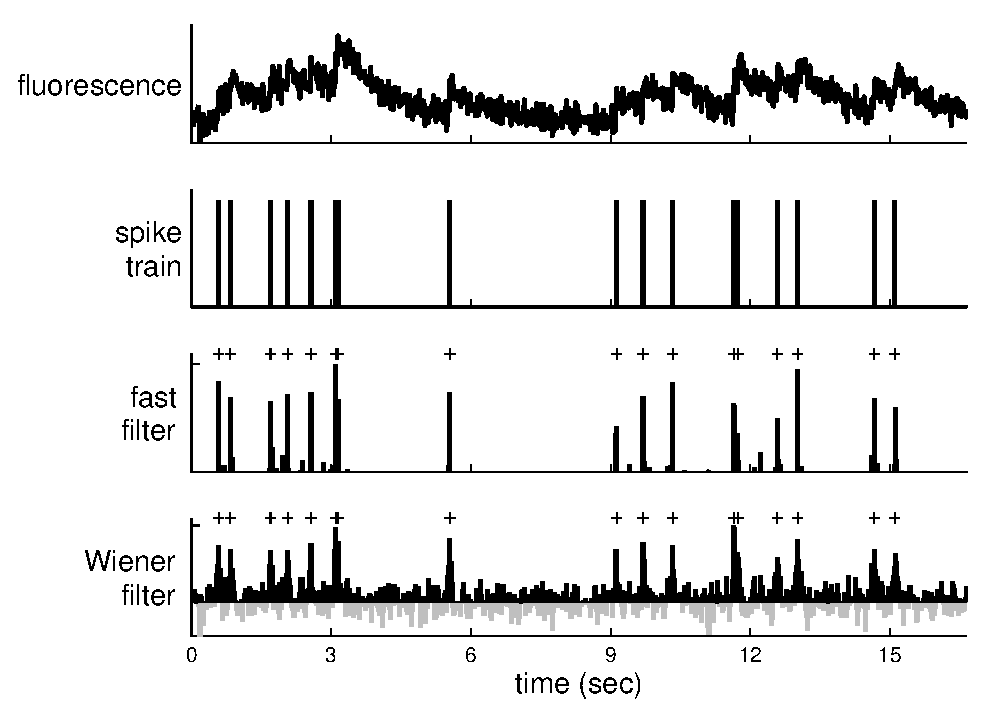
\includegraphics[width=.9\linewidth]{/Users/joshyv/Research/oopsi/fast-oopsi/figs/woopsi_inf}
\caption[\foopsi filter outperforms Wiener filter]{The \foopsi filter significantly outperforms the optimal linear deconvolution (aka, Wiener filter) on typical simulated data. Top panel: fluorescence trace.  Second panel: spike train.  Third panel: \foopsi filter inference.  Bottom panel: Wiener filter inference.  Note that the gray bars indicate \emph{negative} spikes, which, of course, are meaningless. Black '$+$'s in bottom two panels indicate true spike times.  Simulation details: $T=2930$ time steps, $\Del=5$ msec, $\alpha=1$, $\beta=0$, $\sig=0.3$, $\tau=1$ sec, $\lam=1$ Hz.} \label{fig:woopsi_inf}
\end{figure}


Although in Figure \ref{fig:woopsi_inf} the model parameters were provided, in the general case, the parameters are unknown, and must therefore be estimated from the observations (as described in section \ref{sec:learn}). Importantly, estimating the parameters in this ``unsupervised'' manner obviates the need to conduct joint imaging and electrophyiological experiments to obtain ``training'' data.  Figure \ref{fig:woopsi_learn} shows another simulated example; in this example, however, the parameters are estimated from the observed fluorescence trace alone.  Again, it is clear that the \foopsi filter far outperforms the Wiener filter.

\begin{figure}[h!]
\centering 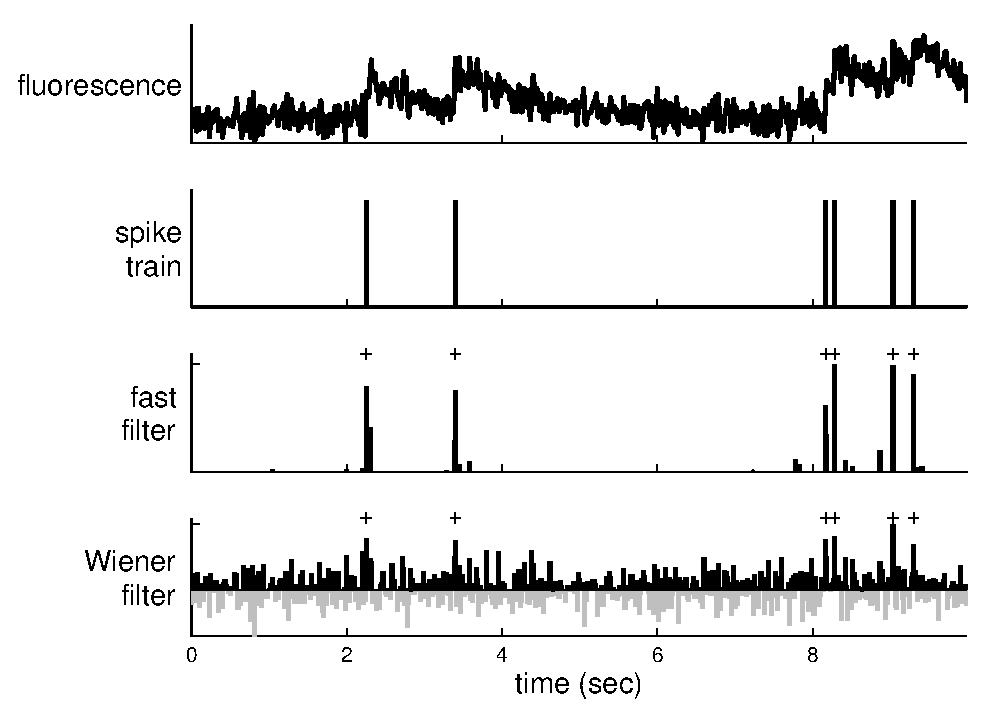
\includegraphics[width=.9\linewidth]{/Users/joshyv/Research/oopsi/fast-oopsi/figs/woopsi_learn}
\caption[parameters may be estimated using the \foopsi filter]{The \foopsi filter significantly outperforms the Wiener filter, even when estimating the parameters only from the observed simulated data.  Simulation details as in Figure \ref{fig:woopsi_inf}.} \label{fig:woopsi_learn}
\end{figure}

Given the above two results, the \foopsi filter was applied to real data.  More specifically, by jointly recording electrophysiologically and imaging, the true spike times are known, and the accuracy of the two filters can be compared.  Figure \ref{fig:woopsi_data} shows a result typical of the 12 joint electrophysiological and imaging experiments conducted. Note that the first few ``events'' are actually pairs of spikes, which is reflected in the inferred spike trains. This suggests that although the scale is arbitrary, the \foopsi filter can correctly ascertain the number of spikes within spike events.  

\begin{figure}[h!]
\centering 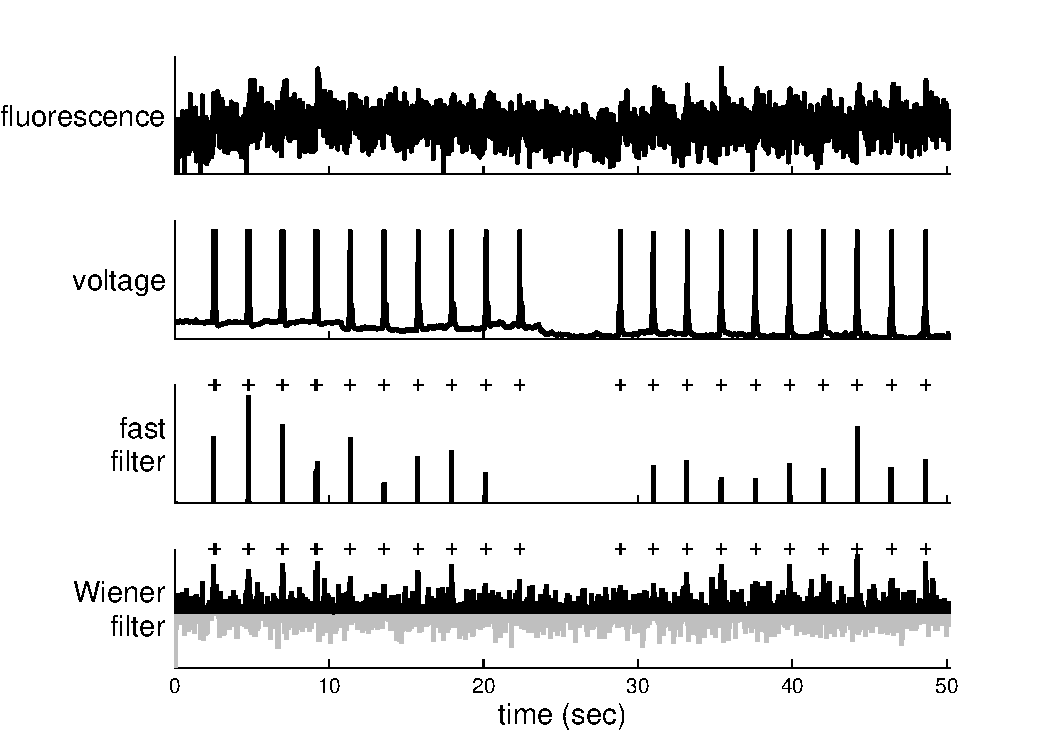
\includegraphics[width=.9\linewidth]{/Users/joshyv/Research/oopsi/fast-oopsi/figs/woopsi_data4}
\caption[\foopsi filter outperforms Wiener filter on real data]{The \foopsi filter significantly outperforms the Wiener filter on typical in vitro data, using Fura-2.  Note that all the parameters for both filters were estimated from the fluorescence data alone (ie, not considering the voltage data at all).} \label{fig:woopsi_data}
\end{figure}

Figure \ref{fig:woopsi_data_doublets} further evaluates this claim.  The cell was forced to spike in ``doublets'' for each spiking event, meaning that the algorithm never saw a single spike event.  Na\"{i}vely, this would suggest that a purely linear approach would struggle to resolve spike fidelity in this high frequency spiking regime.  However, the \foopsi filter correctly identifies nearly all spiking events as ``doublets''.  On the contrary, there is no obvious way to count the number of spikes within each event upon using the Wiener filter.

\begin{figure}[h!]
\centering 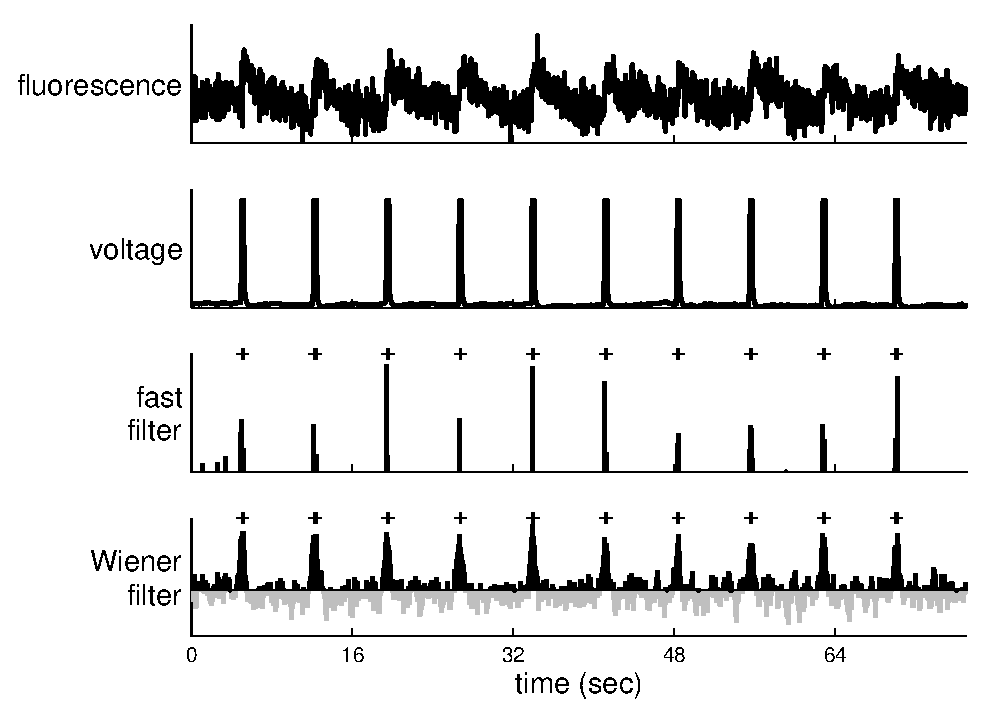
\includegraphics[width=.9\linewidth]{/Users/joshyv/Research/oopsi/fast-oopsi/figs/woopsi_data5}
\caption[\foopsi filter outperforms Wiener filter on doublets]{The \foopsi filter can resolve a sequence of doublets, even in the absence of ever seeing an individual spike.  It is difficult, if not impossible, to count the number of spikes given the Wiener filter output.  Recording and fitting parameters as in Figure \ref{fig:woopsi_data}} \label{fig:woopsi_data_doublets}
\end{figure}






\subsection{Online analysis of spike trains using the \foopsi filter}

A central aim for this work was the development of an algorithm that infers spikes fast enough to use online while imaging a large population of neurons (eg, $\approx 100$).  Figure \ref{fig:pop} shows a segment of the results of running the \foopsi filter on 136 neurons, recorded simultaneously, as described in section \ref{sec:exp}.  Note that the filtered fluorescence signals show fluctuations in spiking much more clearly than the unfiltered fluorescence trace. These spike trains were inferred in super-real-time, meaning that one could infer spike trains for the past experiment while conducting the subsequent experiment. More specifically, a movie with 5,000 frames of 100 neurons can be analyzed in about ten seconds on a standard desktop computer.  Thus, if that movie was recorded at 50 Hz, while collecting the data required 100 seconds, inferring spikes only required ten seconds, a ten-fold improvement over real-time.  


\begin{figure}[h!]
\begin{centering} 
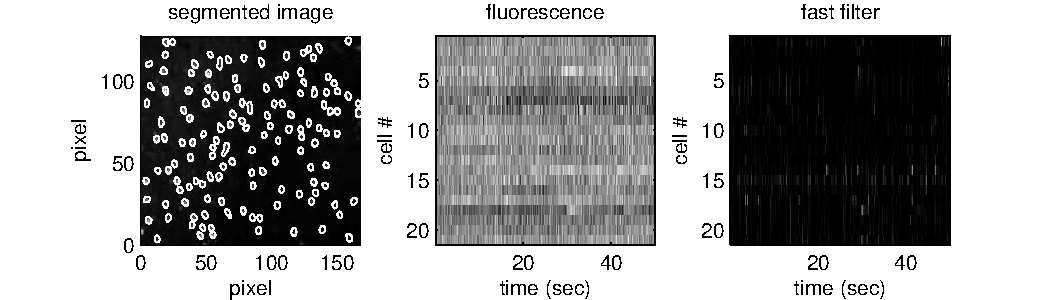
\includegraphics[width=1\linewidth]{/Users/joshyv/Research/oopsi/fast-oopsi/figs/pop}
\end{centering}
\caption[\foopsi filter is robust and works online for populations of neurons]{The \foopsi filter infers spike trains from a large population of neurons imaged simultaneously in vitro, using OBG-1, in super-real-time.  The inferred spike trains convey much more clearly the neural activity.  Left panel: Mean segmented image field.  Middle panel: example fluorescence traces.  Right panel: \foopsi filter output corresponding to each associated trace.} \label{fig:pop}
\end{figure}


\subsection{Extensions}

Section \ref{sec:model} describes a simple principled first-order model relating the spike trains to the fluorescence trace. A number of the simplifying assumptions can be straightforwardly relaxed, as described below.


\subsubsection{Replacing Gaussian observations with Poisson}

In the above, observations were assumed to have a Gaussian distribution.  The statistics of photon emission and counting, however, suggest that a Poisson distribution would be more natural \cite{SjulsonMiesenbock07}, yielding:
\begin{align} \label{eq:poiss}
	F_t \overset{iid}{\sim}\text{Poisson}(\alpha C_t + \beta).
\end{align}
One advantage to this model, over the Gaussian one, besides accuracy, is that the variance parameter no longer exists, which might make learning the parameters simpler.  Importantly, the posterior is still concave in $\bC$, so the same techniques can be used for this model (which requires analytically calculating the gradient and Hessian for the likelihood term implied by Eq.~\eqref{eq:poiss}).  In practice, modifying the filter for this model extension did not seem to improve inference results in any simulations or data (not shown).

\subsubsection{Allowing for a time-varying prior}

In Eq.~\eqref{eq:n}, the rate of spiking is a constant.  Often, additional knowledge about the experiment, including external stimuli, or other neurons spiking, can provide strong time-varying prior information.  A simple model modification can incorporate that feature:
\begin{align}
	n_t &\overset{iid}{\sim} \text{Poisson}(\lam_t \Del),
\end{align}
where $\lam_t$ is now a function of time.  Approximating this time-varying Poisson with a time-varying exponential (as in Eq.~\eqref{eq:obj}) yields a log-concave problem again, so the same techniques can be used to find the most likely spike train, give this prior.  However, as above, this model extension did not yield any improved filtering results (not shown).

\subsubsection{Saturating fluorescence}

Although all the above models assumed a \emph{linear} relationship between $F_t$ and $C_t$, the relationship between fluorescence and calcium is typically better approximated by the nonlinear Hill equation \cite{PologrutoSvoboda04}. Modifying Eq.~\eqref{eq:F} to reflect this change yields: 
\begin{align}
	F_t &= \alpha \frac{C_t}{C_t+k_d} + \beta +  \sig \varepsilon_t, \qquad \varepsilon_t \overset{iid}{\sim} \mN(0,1).
\end{align}
Incorporating this nonlinearity breaks the log-concavity of the posterior, meaning that converging to the global maximum is no longer guaranteed.  Assuming a good initialization can be found, however, if this model is more accurate, then ascending the gradient for this model might yield improved inference results.  In practice, initializing with the linear solution often resulted in nearly equally accurate inference, but this nonlinear inference was far less robust than the inference assuming the linear model (not shown).  
%Unfortunately, using this more powerful model did not result in substantial inference improvements for simulated or in vitro data (not shown).  This is possibly due to approximating the Poisson distribution governing spiking with an exponential distribution.  This approximation is required to ensure concavity of the posterior.  

\subsubsection{Using the \foopsi filter to initialize the SMC filter}

A previously proposed sequential Monte Carlo (SMC) method to infer spike trains can incorporate this nonlinearity, as well as the other model extensions discussed above \cite{VogelsteinPaninski09} . However, this SMC filter is not nearly as efficient as the fast filter proposed here.  Like the \foopsi filter, the SMC filter estimates the model parameters in a completely unsupervised fashion, ie, from the fluorescence observations, using an expectation-maximization algorithm (which requires iterating between computing the expected value of the hidden variables --- $\bC$ and $\bn$ --- and updating the paramters).  In \cite{VogelsteinPaninski09}, parameters for the SMC filter were initialized based on other data.  While effective, this initialization was often far from the final estimates, and therefore, required a relatively large number of iterations (eg, 20--25) before converging.  Thus, it seemed that the \foopsi filter could be used to obtain an improvement to the initial parameter estimates, reducing the required number of iterations.  Indeed, Figure \ref{fig:smc_init} shows how the SMC filter outperforms the \foopsi filter on in vitro data, and only required 3--5 iterations to converge on this data (which was typical).  Note that the first few events of the spike train are individual spikes, resulting in relatively small fluorescence fluctuations, whereas the next events are actually spike doublets or triplets, causing a much larger fluorescence fluctuation.  Only the SMC filter picks up the individual spikes in this trace, a result typical when the effective signal-to-noise ratio (SNR) is so poor.  Thus, these two inference algorithms are complementary: the \foopsi filter can be used for rapid, online inference, and for initializing the SMC filter, which can then be used to further refine the spike train estimate.  Importantly, although the SMC filter often outperforms the \foopsi filter, the \foopsi filter is more robust, meaning that it more often works ``out-of-the-box''.

\begin{figure}[h!]
\centering 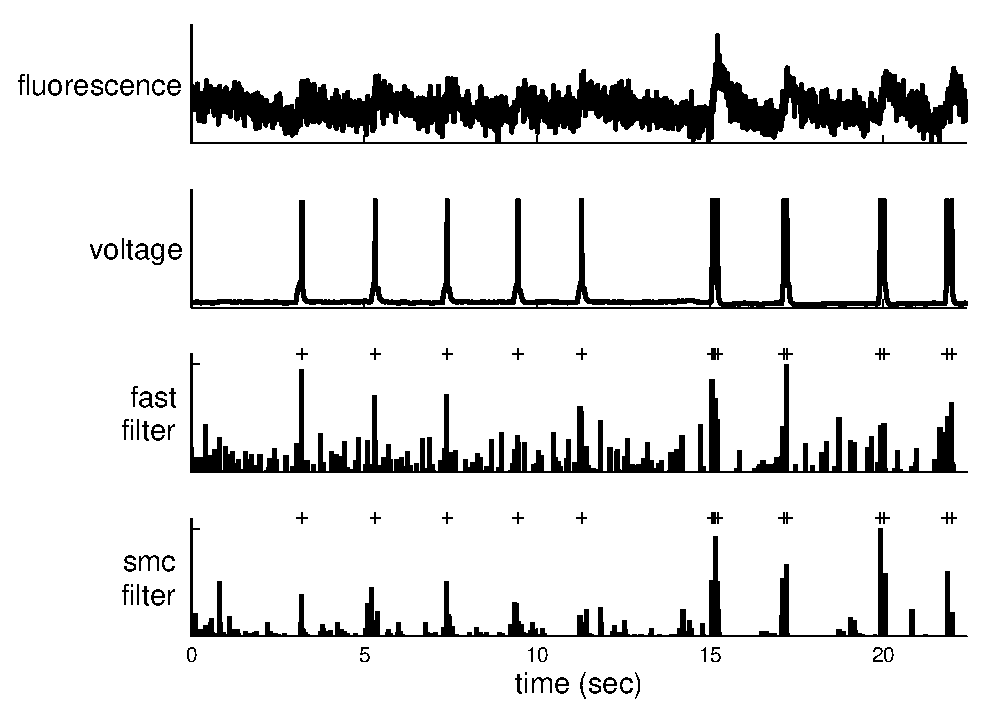
\includegraphics[width=.9\linewidth]{/Users/joshyv/Research/oopsi/fast-oopsi/figs/smc_init12}
\caption[\foopsi filter can initialize Wiener filter]{The \foopsi filter effectively initializes the parameters for the SMC filter (which outperforms the \foopsi filter), significantly reducing the number of expectation-maximization iterations to convergence, on typical in vitro data, using Fura-2.  Note that the ordinate on the bottom panel corresponds to the inferred probability of a spike having occurred in each frame.} \label{fig:smc_init}
\end{figure}

\subsection{Spatial filter} \label{sec:results:spatial}

In the above, the filters operated on one-dimensional fluorescence traces. Typically, although the data are time-series of images which are first segmented into regions-of-interest (ROI), and then (usually) averaged to obtain $F_t$.  In theory, one could improve the effective SNR of the fluorescence trace by scaling each pixel relative to one another.  In particular, pixels not containing any information about calcium fluctuations can be ignored, and pixels that are partially anti-correlated with one another could have weights with opposing signs.  

Figure \ref{fig:spatial} demonstrates the potential utility of this approach.  The top row shows different depictions of an ROI containing a single neuron.  On the far left panel is the true spatial filter for this neuron.  This particular spatial filter was chosen based on experience analyzing both in vitro and in vivo movies; often, it seems that the pixels immediately around the soma are anti-correlated with those in the soma.  This effect is possibly due to the influx of calcium from extracellular space immediately around the soma.  The simulated movie is relatively noisy, as indicated by the second panel, which depicts an exemplary image frame.  The standard approach, given such a noisy movie, would be to first segment the movie to find an ROI corresponding to the soma of this cell, and then spatially average all the pixels found to be within this ROI.  The third panel shows this ``typical spatial filter''.  The fourth panel shows the mean frame.  Clearly, this mean frame is very similar to the true spatial filter.  

The bottom panels of Figure \ref{fig:spatial} depict the effect of using the true spatial filter, versus the typical one. The left side shows the fluorescence trace and its associated spike inference obtained from using the typical spatial filter.  The right side shows the same when using the true spatial filter.  Clearly, the true spatial filter results in a much cleaner fluorescence trace and spike inference.  When the true spatial filter is a single Gaussian, the typical spatial filter works about as well as the true one (not shown).


\begin{figure}[h!]
\centering 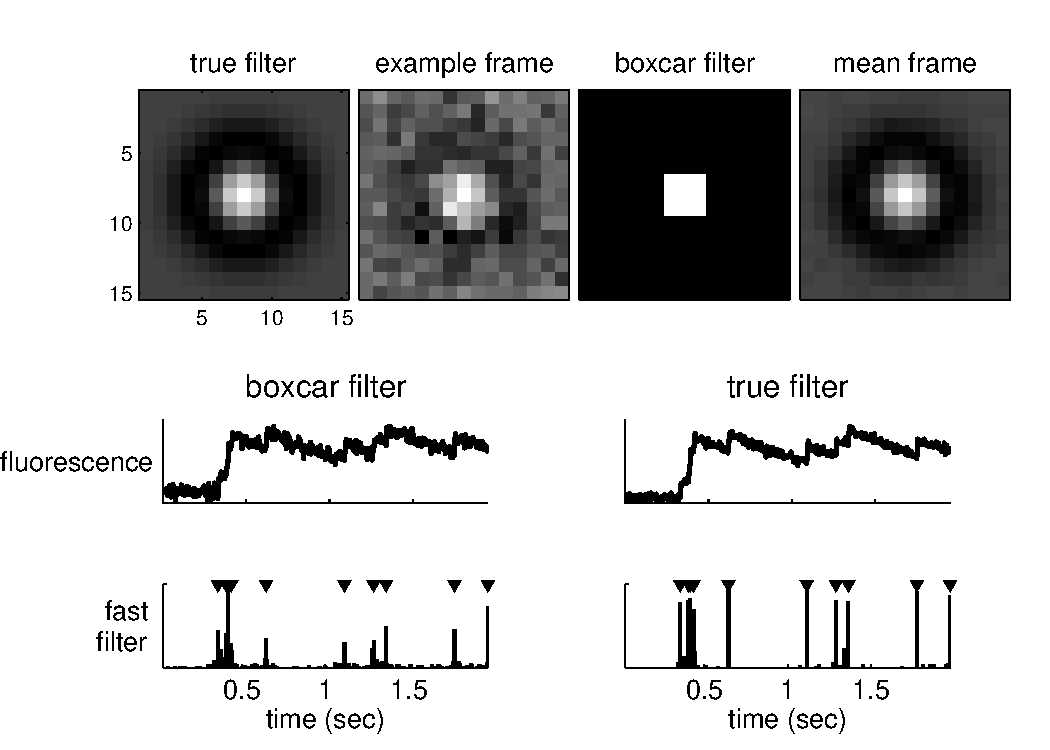
\includegraphics[width=.9\linewidth]{/Users/joshyv/Research/oopsi/fast-oopsi/figs/spatial2}
\caption[spatial filtering can improve effective SNR]{A simulation demonstrating that using a better spatial filter can significantly enhance the effective SNR (see Supplementary Movie 1 for the full movie associated with this simulation). The true spatial filter was a sum of Gaussians: a positively weighted small variance Gaussian, and a negatively weighted large variance Gaussian (both with the same mean).  Top row far left: true spatial filter.  Top row second from left: example frame (frame number 100). Top row second from right: typical spatial filter.   Top row far right: mean frame.  Middle row left: fluorescence trace using typical spatial filter. Bottom row left: \foopsi filter output using typical spatial filter.  Middle row right: fluorescence trace using true spatial filter.  Bottom right: \foopsi filter output using true spatial filter. Simulation details: $\valpha=\mN(\ve{0},2 \bI)-1.1 \mN(\ve{0},2.5 \bI)$ where $\mN(\ve{\mu},\ve{\Sig})$ indicates a Gaussian with mean $\ve{\mu}$ and covariance matrix $\ve{\Sig}$, $\bbeta=1$, $\tau=0.85$ sec, $\lam=5$ Hz.} \label{fig:spatial} 
\end{figure}



\subsection{Overlapping spatial filters} \label{sec:results:overlapping}


The above shows that if a ROI contains only a single neuron, the effective SNR can be enhanced by spatially filtering.  However, this analysis assumes that only a single neuron is in the ROI.  Often, neural spatial filters are overlapping, or nearly overlapping, making the segmentation problem even more difficult.  Therefore, it is desirable to have an ability to crudely segment, yielding only a few neurons in each ROI, and then spatially filter within each ROI to pick out the spike trains from each neuron.  This may be achieved in a principled manner by generalizing the model as described in section \ref{sec:methods:overlapping}.  Figure \ref{fig:spatial_multi_inf} shows how this approach can separate the two signals, assuming that the spatial filters of the two neurons is known.  %Note that the spatial filters are sufficiently overlapping that some ``bleed-though'' can be seen across the traces.  
%While Figure \ref{fig:spatial_multi_inf} shows that one could separate the signals if the spatial filters of the neurons were known, 
Figure \ref{fig:spatial_multi_learn} shows that the spatial filters can be estimated using only the fluorescence movie, by using the approach described in section \ref{sec:methods:overlapping}.


\begin{figure}[h!]
\centering 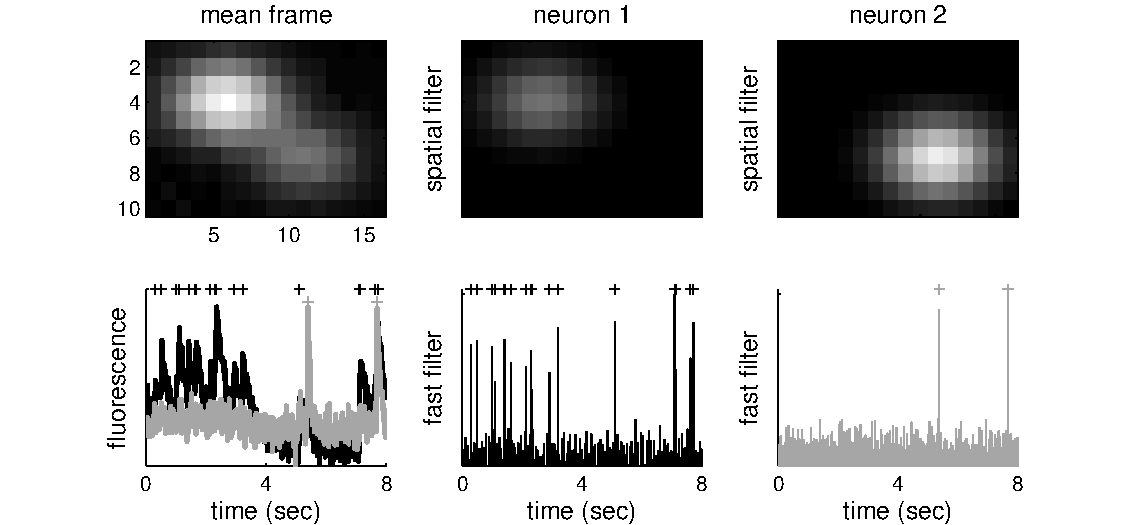
\includegraphics[width=.9\linewidth]{/Users/joshyv/Research/oopsi/fast-oopsi/figs/spatial_multi_inf}
\caption[overlapping spatial filters are not problematic]{Simulation showing that even when two neurons' spatial filters are overlapping, one can separate the two signals by spatial filtering. Simulation details: $\valpha^1=\mN([-1.8 1.8],2 \bI)\, \valpha^2=\mN([1.8 -1.8],5 \bI)$, $\bbeta=[1 1]\T$, $\tau=[0.5 0.5]\T$ sec, $\lam=[1.5 1.5]$ Hz.} \label{fig:spatial_multi_inf}
\end{figure}



\begin{figure}[h!]
\centering 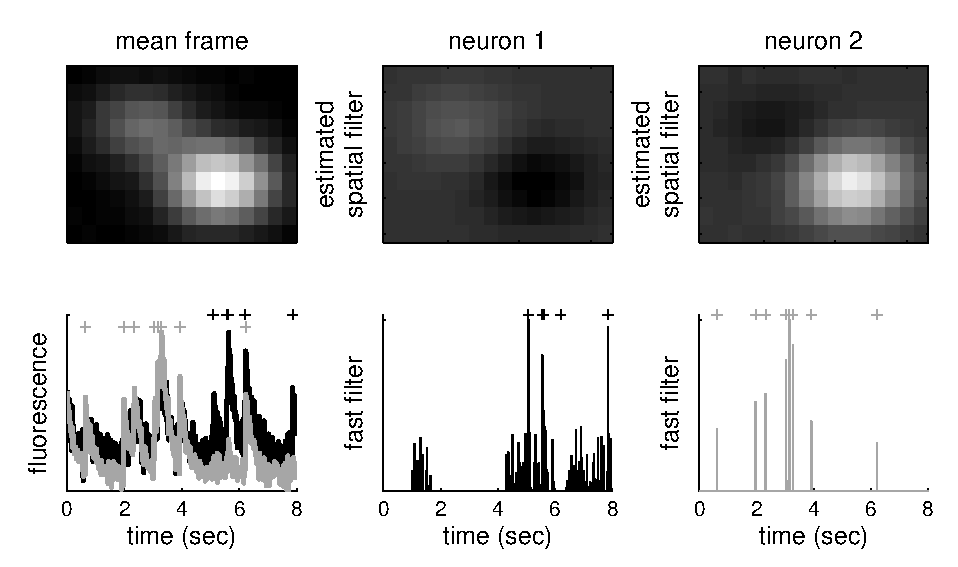
\includegraphics[width=.9\linewidth]{/Users/joshyv/Research/oopsi/fast-oopsi/figs/spatial_multi_learn}
\caption[overlapping spatial filters can be estimated]{Simulation showing that even when two neuron's spatial filters are largely overlapping, linearly scaled estimates of the spatial filter of each neuron can be inferred, to separate the two signals. Simulation details as above.} \label{fig:spatial_multi_learn}
\end{figure}





\section{Discussion} \label{sec:dis}

% \paragraph{Summary}

This work describes an algorithm that approximates the \emph{maximum a posteriori} (MAP) spike train, given a fluorescence movie.  The approximation is required because finding the actual MAP estimate is not currently computationally tractable.  Replacing the assumed Poisson distribution on spikes with an exponential distribution yields a log-concave optimization problem, which can be solved using standard gradient ascent techniques (such as Newton-Raphson).  This exponential distribution has an advantage over a Gaussian distribution by restricting spikes to be positive, which improves inference quality (c.f. Figure \ref{fig:woopsi_inf}), and is a better approximation to a Poisson distribution with low rate.  %This result is common within machine learning \cite{Hoyer04,OGradyPearlmutter06}: imposing a non-negative constraint often helps prevent oscillations and other overfitting artifacts. This non-negative constraint is enforced by interior-point methods.  
Furthermore, by utilizing the special structure of the Hessian matrix (ie, it is tridiagonal), this approximate MAP spike train can be inferred fast enough on standard computers to use it for online analyses.  Finally, all the parameters can be estimated from only the fluorescence observations, obviating the need for joint electrophysiology and imaging (c.f. Figure \ref{fig:woopsi_learn}).  This approach is robust, in that it works ``out-of-the-box'' on all the in vivo and in vitro data analyzed (c.f. Figure \ref{fig:woopsi_data}).

%This work is closely related to several previously proposed algorithms.  
Ideally, one could compute the full joint posterior of entire spike trains, conditioned on the fluorescence data.  This distribution is analytically intractable, due to the Poisson assumption on spike trains.  A Bayesian approach could use Markov Chain Monte Carlo to recursively sample spikes until a whole sample spike train is obtained \cite{AndrieuDoucet01,MishchenkoPaninski09}.  Because a central aim here was computational expediency, a ``greedy'' approach is natural: ie, recursively sample the most likely spike, update the posterior, and repeat until the posterior stops increasing.  Template matching, projection pursuit regression \cite{FS81}, and matching pursuit \cite{MallatZhang93} are examples of such a greedy approach (Greenberg et al's algorithm could also be considered a special case of such a greedy approach).  Both the greedy methods, and the one developed here, aim to optimize a similar objective function.  While greedy methods reduce the computational burden by restricting the search space of spike trains, here analytic approximations are made.  The advantage of the greedy approaches relative to this one is that they result in a spike train (ie, a binary sequence), whereas the approach developed herein is guaranteed to be approximately optimal, given the model.  


Because this filter is model based, it can be generalized in several ways to improve accuracy.  Unfortunately, some of these generalizations do not improve inference accuracy, probably because of the exponential approximation.  Instead, the \foopsi filter output can be used to initialize the SMC filter \cite{VogelsteinPaninski09}, to further improve inference quality (c.f. Figure \ref{fig:smc_init}).  Another model generalization allows incorporation of spatial filtering of the raw movie into this approach (c.f. Figure \ref{fig:spatial}).  The parameters of the spatial filter can be estimated from the data, even when spatial filters are overlapping (c.f. Figure \ref{fig:spatial_multi_learn}).

A number of extensions follow from this work.  First, further development on some of the model generalizations may improve inference results. Second, pairing this filter with a crude but automatic segmentation tool to obtain ROIs would create a completely automatic algorithm that converts raw movies of populations of neurons into populations of spike trains.  Third, combining this algorithm with recently developed connectivity inference algorithms on this kind of data \cite{MishchenkoPaninski09}, could yield very efficient connectivity inference.